Una vez introducido el diseño general del sistema, en este capítulo se explicarán los agentes especializados que acceden a las fuentes de datos del proyecto software. 

Para ello primero se introducirá la estructura de la base común \opus{SpecializedAgent}, tras lo que se detallarán tanto las herramientas como el grafo de los cinco agentes especialistas que extienden esta base.

\section{Estructura SpecializedAgent}
El grafo común de este agente se divide en tres pasos generales; la configuración del prompt inicial a utilizar mediante la función \opus{prepare_prompt()} heredada de \opus{BaseAgent}, la ejecución de un subgrafo que implementa el patrón ReAct (Véase Sección \ref{}) y la ejecución de un agente resumidor en caso de ser necesario. La ejecución del grafo general se ilustra en la Figura \ref{fig:specialized}.

\begin{figure}[h]
  \centering
  \adjustbox{center=\textwidth}{\hspace{-1.2cm}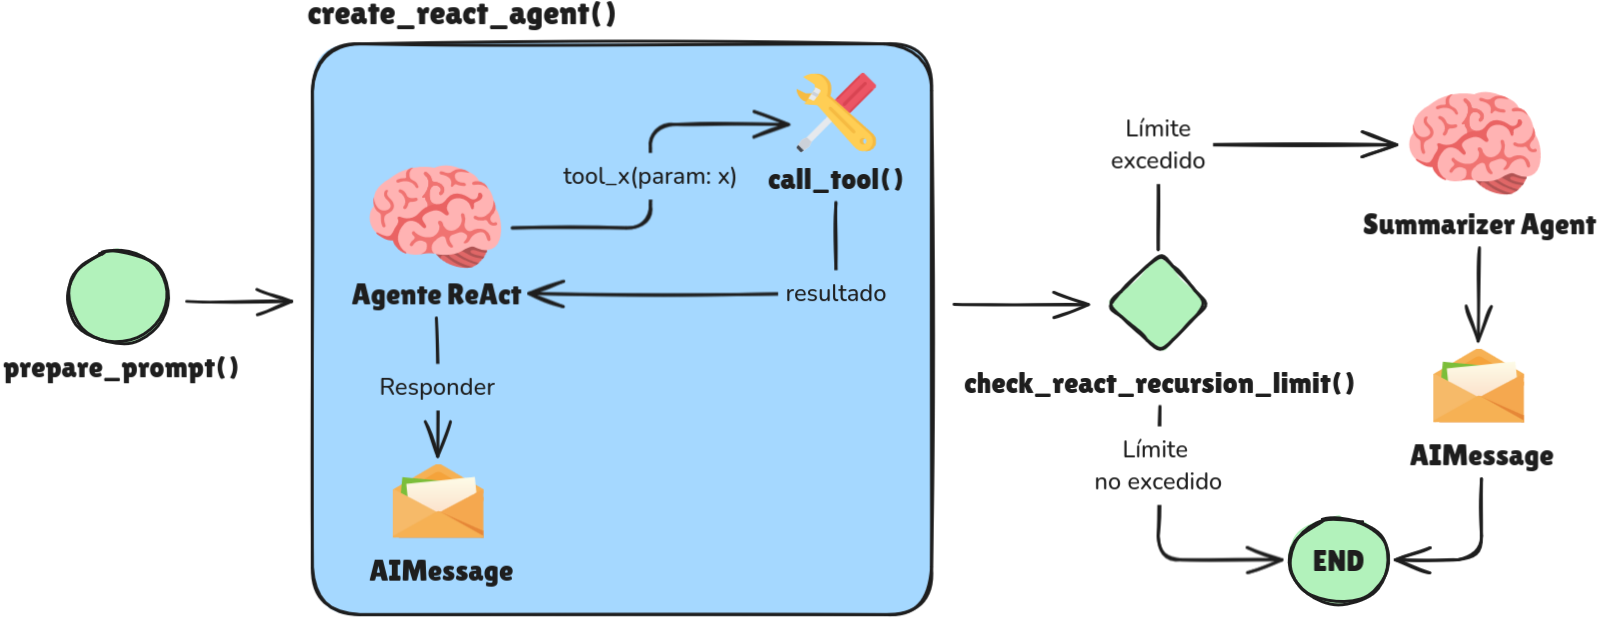
\includegraphics[width=1.3\linewidth]{figures/specialized.png}}
  \caption{Grafo de ejecución de agentes especializados}
  \label{fig:specialized}
\end{figure}

El grafo ReAct se ha implementado utilizando el agente prefabricado \opus{create_react_agent()} de LangGraph. Este agente acepta una serie de herramientas y un prompt inicial y entra en un bucle de ejecución en el que el agente llama a herramientas y observa su resultado. El grafo finaliza su ejecución cuando el mensaje del agente no contiene llamadas a herramientas, es decir, cuando contiene la respuesta final. 

Se ha establecido un límite de iteraciones que el grafo ReAct puede ejecutar, ya que se ha observado que en ocasiones entra en un bucle de ejecución excesivamente extenso al no encontrar la información requerida. De esta forma, en caso de llegar al límite de iteraciones, un agente resumdidor intenta generar una respuesta con la información disponible observando todas las ejecuciones de las herramientas. En el Listado \ref{lst:spec_graph} se ilustra la función que define el grafo explicado.

\begin{lstlisting}[caption={\protect\opus{create_graph: Grafo de agentes especializados} },label={lst:spec_graph}]
  def create_graph(self) -> CompiledGraph:
      # Crear grafo ReAct
      agent_tools = self.get_agent_tools()
      self.react_graph = create_react_agent(
          model=self.model,
          tools=agent_tools,
          checkpointer=self.checkpointer
      )

      # Crear grafo del SpecializedAgent
      graph_builder = StateGraph(AgentState)

      # Añadir nodos 
      graph_builder.add_node("prepare", self.prepare_prompt)
      graph_builder.add_node("react", self.call_langgraph_react_graph)
      graph_builder.add_node("response_summarizer", self.generate_summarized_response)

      # Establecer flujo entre nodos 
      graph_builder.set_entry_point("prepare")
      graph_builder.add_edge("prepare", "react")
      graph_builder.add_conditional_edges("react", self.check_react_recursion_limit)

      return graph_builder.compile()
\end{lstlisting}

Para acceder al estado de ejecución del agente ReAct tras finalizar abruptamente su ejecución por el límite de mensajes, se ha utilizado el sistema de autoguardado de LangGraph. Para ello, en la inicialización del agente se crea un objeto \opus{AsyncPostgresSaver}, vinculado tanto a la base de datos PostgreSQL mediante un \textit{Pool} de conexión asíncrono \ref{} como al contexto de cierre asíncrono \opus{global_exit_stack}. De esta forma, se guardan en una collección de Postgres todos los estados de ejecución, y se pueden acceder indicando su identificador. El uso del guardador asíncrono evita problemas de concurrencia al ejecutar varios agentes asíncronos. 

\subsection{Gestión de herramientas}

Algunas herramientas proporcionadas por los servidores MCP son innecesarias o contraproducentes para algunos agentes. Para evitar incluir en el prompt de los agentes contenido innecesario, se debe indicar al instanciar un agente el nombre de las herramientas que se van a utilziar, para posteriormente filtrar las herramientas en el cliente. 

Adicionalmente, algunos servidores MCP no proporcionan todas las funcionalidades necesarias. Para obtener estas herramientas adicionales, la función \opus{add_additional_tools()} añade en cada caso herramientas adicionales de ser necesario. 

\section{Agentes implementados}
En esta sección se detallarán los cinco agentes desarrollados que extienden las funcionalidades explicadas en la sección anterior.

\subsection{Agente código}
Para obtener información sobre el código fuente del repositorio del proyecto software, el flujo de este agente sigue el siguiente proceso: mediante \opus{prepare_prompt()} se incluye en el prompt del sistema el árbol de directorios del repositorio obtenido con la herramienta \opus{get_repository_tree_tool} y fragemntos de código, denominados \textit{chunks}, relevantes para la consulta actual obtenidos mediante la herramienta \opus{get_code_repository_rag_docs_from_query_tool}. Tras concatenar la consulta al agente mediante un \opus{HumanMessage}, este tiene que decidir si buscar \textit{chunks} adicionales sobre un subdirectorio concreto indicando otra consulta, buscar ficheros específicos con la herramienta \opus{get_file_from_repository_tool} indicando su ruta relativa, o responder directamente a la consulta. 

\subsubsection{Herramientas de acceso a código}
Para implementar las herramientas de este agente, en el componente \opus{servidor_mc_bd_codigo} se han dividido los ficheros del proyecto GitLab en \textit{chunks} y posteriormente se han indexado en la base de datos Postgres.

Para implementar este sistema RAG, se ha utilizado la extensión PGVector sobre PostgreSQL. Dicha extensión ofrece la opción de mezclar vectores embeddings en una tabla SQL tradicional, proporcionando operaciones de búsqueda semántica combinadas con operaciones SQL. Para ello, se ha definido el modelo relacional ilustrado en la Figura \ref{fig:relacional}, implementando el modelo ORM de SQLAlchemy sobre Python. El diseño se basa en una tabla \opus{FileSystem} para cada fichero o directorio, la cual puede contener varios \opus{FileChunk} indexados en la columna \opus{embedding} de tipo \opus{Vector}. Además, cada \textit{chunk} puede referenciar o ser referenciado por otros \textit{chunk}, en caso de que el chunk referenciado contenga una clase o función definida en el chunk referenciador. La tabla \opus{Ancestor} constituye un patrón de tabla de cierre para acceder eficientemente a todos los ficheros dentro de un subdirectorio. 

\begin{figure}[h]
  \centering
  \adjustbox{center=\textwidth}{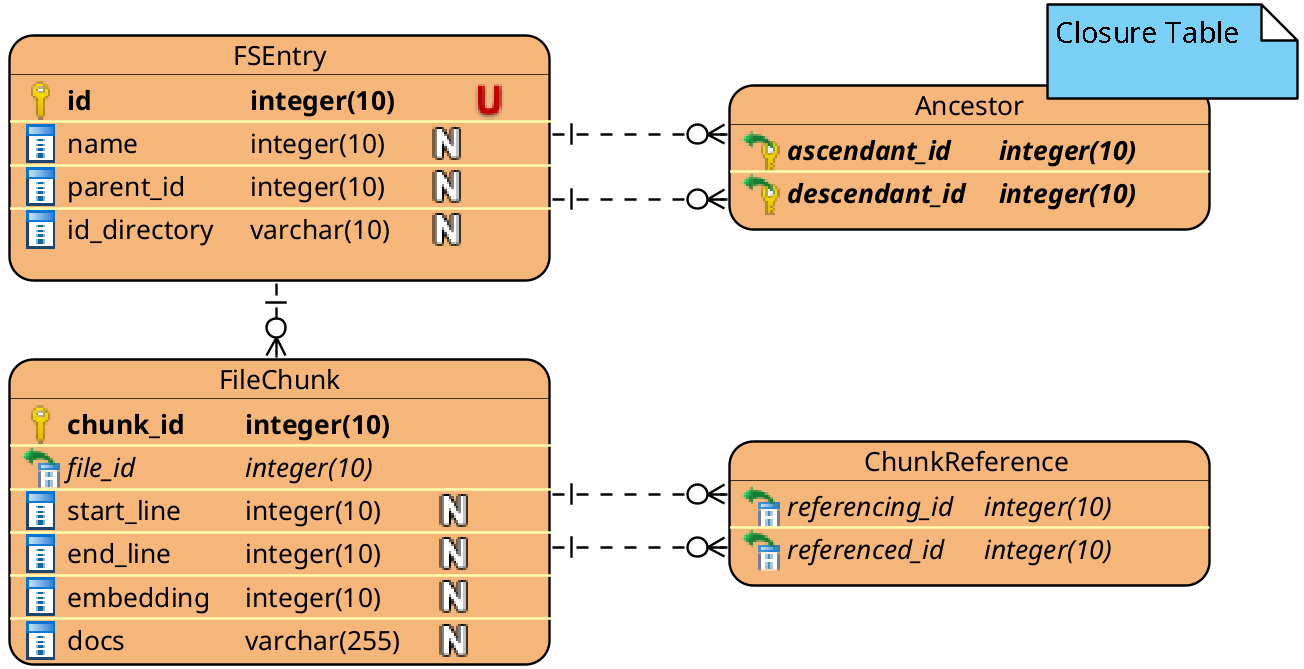
\includegraphics[width=0.95\linewidth]{figures/db.png}}
  \caption{Diagrama relacional de la base de datos con el código fuente del proyecto software}
  \label{fig:relacional}
\end{figure}

\paragraph{División de los segmentos de código}
Para realizar la división de los ficheros en \textit{chunks}, se han considerado las clases y funciones que componen el código. 

\begin{figure}[h]
  \centering
  \adjustbox{center=\textwidth}{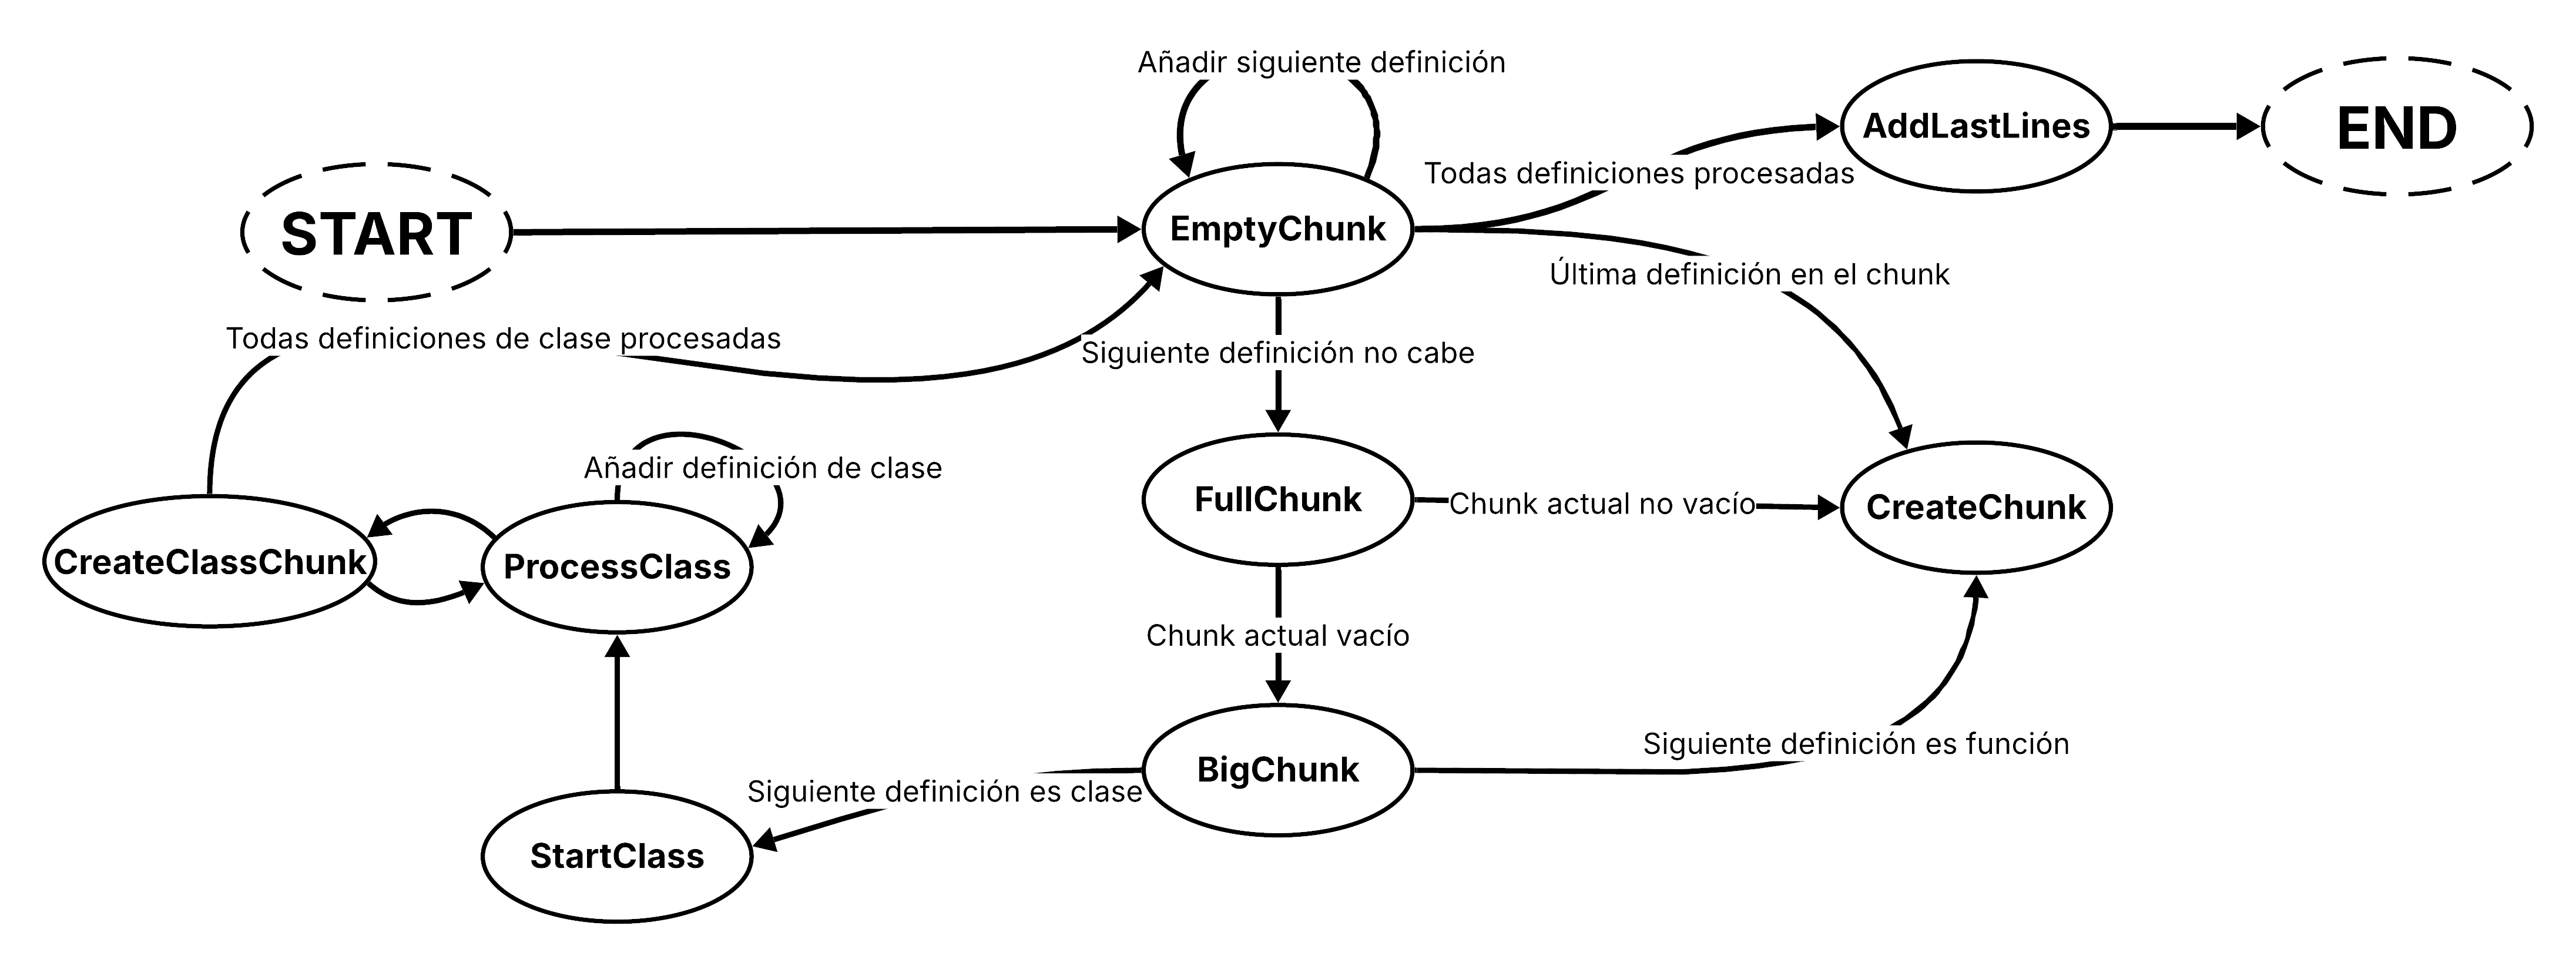
\includegraphics[width=1.35\linewidth]{figures/chunks.png}}
  \caption{Algoritmo de chunking considerando definiciones de funciones y clases en el código fuente}
  \label{fig:chunks}
\end{figure}









